\documentclass[letterpaper,10pt]{article}

%\setlength{\parindent}{0in}
%\usepackage{fullpage} 
\usepackage{amsmath}
\usepackage{amssymb}
\usepackage{enumerate}
\usepackage{graphicx}
\usepackage[table]{xcolor}
\usepackage{dcolumn}
\oddsidemargin 0.0in
\textwidth 6.5in
\newcolumntype{.}{D{.}{.}{-1}}
\newcommand*{\myalign}[2]{\multicolumn{1}{#1}{#2}}

%opening
\title{Homework}
\author{Steve Mazza}
%\date{July 22, 2013}

\begin{document}
\maketitle

\section*{Midterm Project}
\subsection*{Problem 1}
\subsubsection*{(a)}
\subsubsection*{(b)}
\subsubsection*{(c)}
\subsubsection*{(d)}

\subsection*{Problem 2}
\subsubsection*{(a)}
\subsubsection*{(b)}
\subsubsection*{(c)}
\subsubsection*{(d)}
\subsubsection*{(e)}
\subsubsection*{(f)}
\subsubsection*{(g)}

\section*{Homework 7}
\subsection*{Problem 1}
Root-locus plots of the following functions\dots
\subsubsection*{(a)}
\begin{center}
    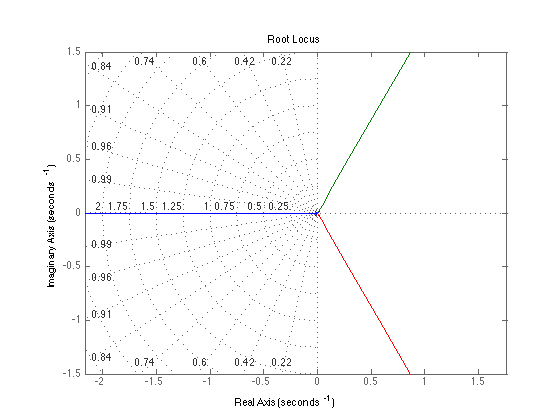
\includegraphics[width=0.6\textwidth]{homework04-7-1-a.png} \\
   $G(s) = \dfrac{1}{(s+0)^{3}}$
\end{center}
\subsubsection*{(b)}
\begin{center}
    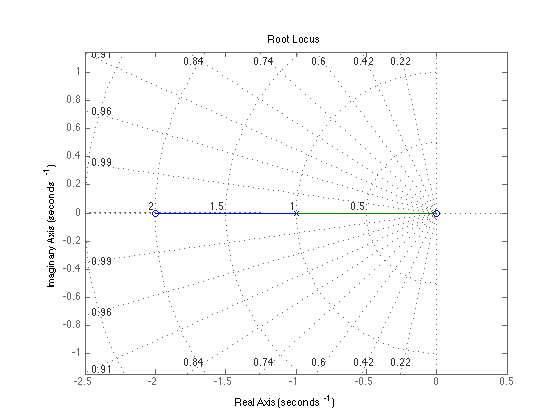
\includegraphics[width=0.6\textwidth]{homework04-7-1-b.png} \\
   $G(s) = \dfrac{(s+0)(s+2)}{(s+1)^{2}}$
\end{center}
\subsubsection*{(c)}
\begin{center}
    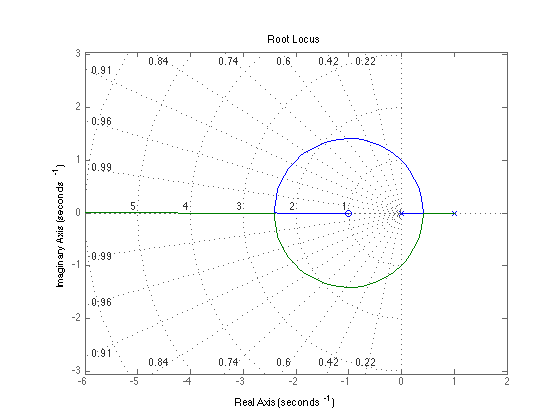
\includegraphics[width=0.6\textwidth]{homework04-7-1-c.png} \\
   $G(s) = \dfrac{s+1}{(s+0)(s-1)}$
\end{center}
\subsubsection*{(d)}
\begin{center}
    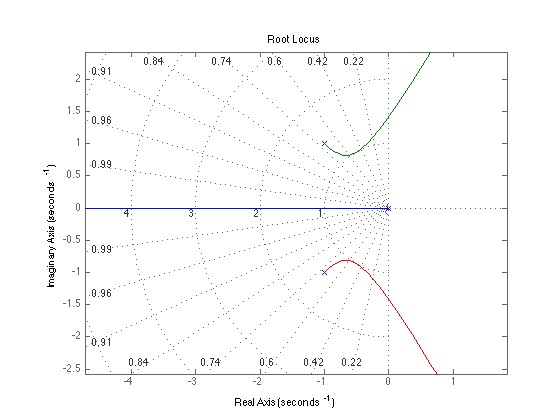
\includegraphics[width=0.6\textwidth]{homework04-7-1-d.png} \\
   $G(s) = \dfrac{1}{(s+0)(s+1+i)(s+1-i)}$
\end{center}
\subsubsection*{(e)}
\begin{center}
    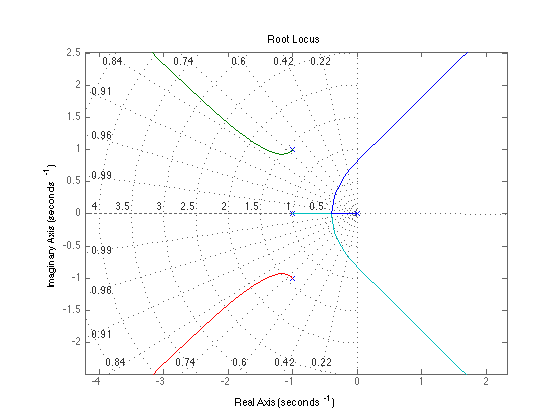
\includegraphics[width=0.6\textwidth]{homework04-7-1-e.png} \\
   $G(s) = \dfrac{1}{(s+0)(s+1+i)(s+1-i)(s+1)}$
\end{center}
\subsubsection*{(f)}
\begin{center}
    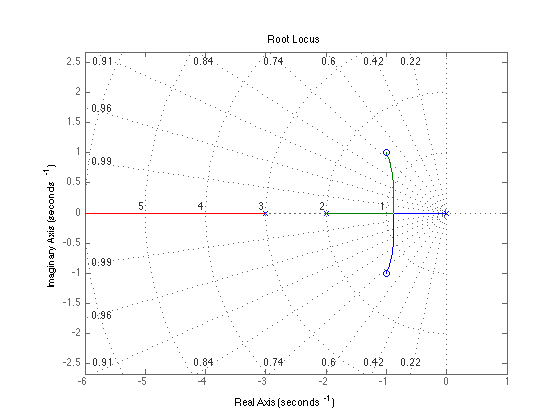
\includegraphics[width=0.6\textwidth]{homework04-7-1-f.png} \\
   $G(s) = \dfrac{(s+1-i)(s+1+i)}{(s+0)(s+2)(s+3)}$
\end{center}
\subsubsection*{(g)}
\begin{center}
    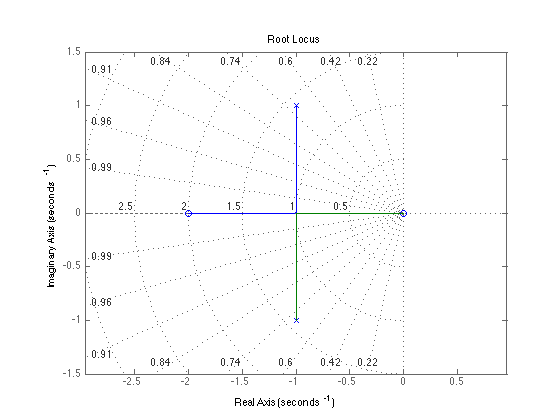
\includegraphics[width=0.6\textwidth]{homework04-7-1-g.png} \\
   $G(s) = \dfrac{(s+0)(s+2)}{(s+1-i)(s+1+i)}$
\end{center}
\subsubsection*{(h)}
\begin{center}
    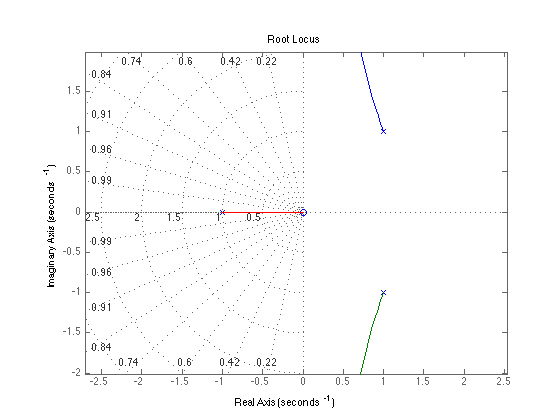
\includegraphics[width=0.6\textwidth]{homework04-7-1-h.png} \\
   $G(s) = \dfrac{(s+0)}{(s+1)(s-1-i)(s-1+i)}$
\end{center}
\subsubsection*{(i)}
\begin{center}
    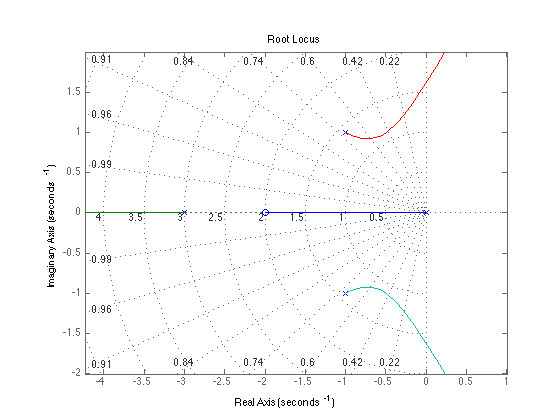
\includegraphics[width=0.6\textwidth]{homework04-7-1-i.png} \\
   $G(s) = \dfrac{(s+2)}{(s+0)(s+3)(s+1-i)(s+1+i)}$
\end{center}

\subsection*{Problem 4}
First we apply our reduction rules to the system as follows:
\begin{align*}
	G(s) &= \dfrac{20}{(s+1)(s+4)} \\
	&= \dfrac{\dfrac{20}{(s+1)(s+4)}}{1+\dfrac{20}{(s+1)(s+4)}\times K} \\
	&= \dfrac{20}{s^{2}+5s+4+20K} \times \dfrac{1}{s} \\
	&= \dfrac{\dfrac{20}{\dfrac{20}{s^{3}+5s^{2}+4s+20Ks}}}{1+\dfrac{20}{s^{3}+5s^{2}+4s+20Ks}} \\
	&= \dfrac{20}{s^{3}+5s^{2}+4s+20Ks+20}
\end{align*}

\subsection*{Problem 5}

\end{document}